\section{Principal Component Analysis (PCA)}\label{sec:pca}

\subsection{Richiami utili}

\begin{nota}{Spettro di una matrice simmetrica}{spettro}
Visto che \( \Sigma \in \mathcal{M}_{n \times n}\) è simmetrica e definita
positiva (come ogni matrice di covarianza), allora:
\begin{itemize}
  \item ammette $n$ autovalori reali e non negativi: \( \lambda_i \geq 0 \);
  \item esiste una base ortonormale di autovettori \( v_i \);
  \item gli autovettori sono ortogonali tra loro;
  \item \( \Sigma v_i = \lambda_i v_i \) equivale a dire che \( \Sigma = V
  \Lambda V^\mathsf{T} \).
\end{itemize}
\end{nota}

\subsection{Definizione}

La \textbf{Principal Component Analysis (PCA)} è una trasformazione lineare che
serve a decorrelare le componenti di un dataset multidimensionale. È
comunemente utilizzata per la riduzione della dimensionalità, il pre-processing
e la visualizzazione.

\begin{definizione}{Componenti principali}{pca}
La PCA consiste nel trovare una base ortonormale nello spazio dei dati tale che:
\begin{itemize}
  \item le nuove coordinate (\emph{componenti principali}) siano incorrelate tra
  loro;
  \item la prima componente abbia la massima varianza possibile;
  \item ogni successiva componente massimizzi la varianza residua, mantenendosi
  ortogonale alle precedenti.
\end{itemize}
\end{definizione}

\subsection{Interpretazione geometrica}

La PCA applica una \textbf{rotazione dello spazio} dei dati centrati (cioè con
media nulla), allineando gli assi principali con le direzioni di massima
varianza. Se \( X \in \mathbb{R}^{n \times d} \) è il dataset centrato:
\[
Y = V^\mathsf{T} X
\]
dove \( V \in \mathbb{R}^{d \times d} \) è la matrice degli autovettori di \(
\Sigma = \mathrm{Cov}(X) \). Le nuove variabili \( Y \) sono scorrelate e
ordinate per varianza decrescente.

\begin{figure}[H]
    \centering
    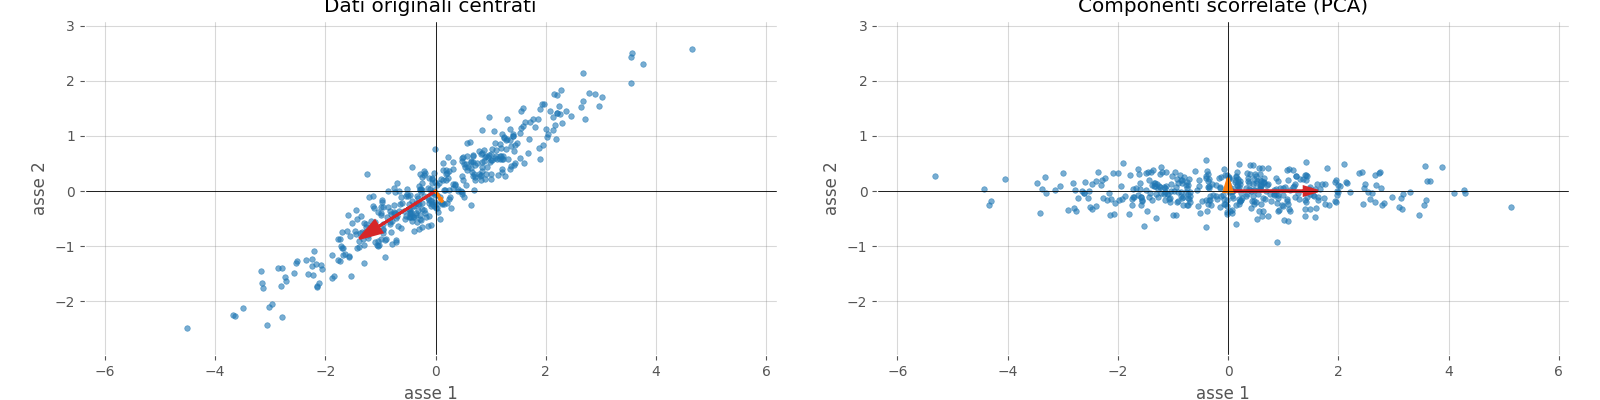
\includegraphics[width=\textwidth]{images/th_10_12/rotation_transformation.png}
    \caption{Esempio di rotazione di un vettore aleatorio bidimensionale. La distribuzione originale centrata (a sinistra) viene ruotata in modo che i suoi assi principali coincidano con le direzioni di massima varianza (a destra).}
    \label{fig:rotation_transformation}
\end{figure}

\subsection{Autovalori e autovettori della covarianza}

\begin{teorema}{Teorema spettrale per la matrice di covarianza}{pca-spettrale}
Sia \( \Sigma \in \mathbb{R}^{d \times d} \) una matrice di covarianza, cioè
reale, simmetrica e definita positiva. Allora esistono:
\begin{itemize}
  \item una base ortonormale di autovettori \( v_1, \dots, v_d \in \mathbb{R}^d
  \);
  \item autovalori reali non negativi \( \lambda_1, \dots, \lambda_d \geq 0 \);
\end{itemize}
tali che:
\[
\Sigma v_k = \lambda_k v_k, \qquad v_j^\mathsf{T} v_k = \delta_{jk}
\]
cioè:
\[
\Sigma = V \Lambda V^\mathsf{T}
\]
dove \( V = [v_1 \; \dots \; v_d] \) è ortogonale e \( \Lambda =
\mathrm{diag}(\lambda_1, \dots, \lambda_d) \).
\end{teorema}

\begin{proposizione}{La matrice degli autovettori è
ortogonale}{pca-matrice-ortogonale}
Sia \( \Sigma \in \mathbb{R}^{d \times d} \) una matrice simmetrica. Siano \(
v_1, \dots, v_d \in \mathbb{R}^d \) autovettori ortonormali di \( \Sigma \), e
si definisca \( V := [v_1 \ \dots \ v_d] \in \mathbb{R}^{d \times d} \). Allora:
\[
V^\mathsf{T} V = I \quad \text{e} \quad VV^\mathsf{T} = I
\]
cioè \( V \) è una matrice ortogonale.
\end{proposizione}

\begin{dimostrazione}{}{dim-pca-matrice-ortogonale}
Osserviamo che l’elemento \( (i, j) \) della matrice \( V^\mathsf{T} V \) si
calcola come:
\[
[V^\mathsf{T} V]_{ij} = \sum_{k=1}^d [V^\mathsf{T}]_{ik} [V]_{kj}
= \sum_{k=1}^d v_{k,i} v_{k,j}
\]

Notiamo che:
\[
\sum_{k=1}^d v_{k,i} v_{k,j} = v_i^\mathsf{T} v_j =
\begin{cases}
1 & \text{se } i = j \\
0 & \text{se } i \neq j
\end{cases}
= \delta_{ij}
\]

Quindi:
\[
V^\mathsf{T} V = I \quad \text{(matrice identità)}
\]

Segue che \( V \) è ortogonale, quindi \( V^\mathsf{T} = V^{-1} \).
Da questo deduciamo anche \( VV^\mathsf{T} = I \), e quindi:
\[
VV^\mathsf{T} = V V^{-1} = I
\]

In conclusione, \( V \) è una rotazione (o riflessione), cioè una
trasformazione ortogonale dello spazio.
\end{dimostrazione}

\begin{proposizione}{Diagonalizzazione spettrale: \texorpdfstring{\( \Sigma V =
V \Lambda \)}{Sigma V = V Lambda}}{pca-spettrale-diretta}
Sia \( \Sigma \in \mathbb{R}^{d \times d} \) una matrice simmetrica, e siano \(
v_1, \dots, v_d \) i suoi autovettori ortonormali associati agli autovalori \(
\lambda_1, \dots, \lambda_d \). Costruiamo:
\[
V := [v_1 \; v_2 \; \dots \; v_d], \quad \Lambda := \mathrm{diag}(\lambda_1,
\dots, \lambda_d)
\]
Allora:
\[
\Sigma V = V \Lambda
\]
\end{proposizione}

\begin{dimostrazione}{}{dim-pca-spettrale-diretta}
    \paragraph{Versione vista a lezione} Verifichiamo che \( \Sigma V = V
    \Lambda \) calcolando il generico elemento \( (i, j) \) di entrambi i
    membri.

A sinistra:
\[
[\Sigma V]_{ij} = \sum_k \Sigma_{ik} V_{kj}
= \sum_k \Sigma_{ik} (v_j)_k = [\Sigma v_j]_i
\]
Poiché \( v_j \) è autovettore di \( \Sigma \), abbiamo:
\[
\Sigma v_j = \lambda_j v_j \quad \Rightarrow \quad [\Sigma v_j]_i = \lambda_j
(v_j)_i = \lambda_j V_{ij}
\]

A destra:
\[
[V \Lambda]_{ij} = \sum_k V_{ik} \Lambda_{kj} = V_{ij} \lambda_j = \lambda_j
V_{ij}
\]

Poiché i due membri coincidono elemento per elemento:
\[
    [V \Lambda]_{ij} = \sum_k V_{ik} \Lambda_{kj} \stackrel{\text{\tiny
    (\(\Lambda_{kj} = 0 \forall k \neq j\))}}{=} V_{ij} \lambda_j = \lambda_j
    V_{ij}
\]

\paragraph{Alternativa}

Abbiamo già verificato che:
\[
\Sigma = V \Lambda V^\mathsf{T} ,\quad V^\mathsf{T}V = VV^\mathsf{T} = I
\]
Moltiplicando ambo i membri della prima equazione per $V$ otteniamo:
\begin{align*}
    \Sigma &= V \Lambda V^\mathsf{T} \\
    \Sigma V &= V \Lambda (V^\mathsf{T} V) \\
    \Sigma V &= V \Lambda
\end{align*}

\end{dimostrazione}

\subsection{PCA e decorrelazione}

\begin{proposizione}{Decorrelazione delle componenti tramite
PCA}{pca-covarianza-diagonale}
Sia \( X \in \mathbb{R}^{d \times n} \) un dataset centrato con matrice di
covarianza \( \Sigma = \mathrm{Cov}(X) \). Sia \( V \in \mathbb{R}^{d \times d}
\) una matrice ortogonale composta dagli autovettori di \( \Sigma \), e sia:
\[
Y = V^\mathsf{T} X
\]
la trasformazione PCA. Allora:
\[
\mathrm{Cov}(Y) = \Lambda
\]
dove \( \Lambda \) è la matrice diagonale degli autovalori di \( \Sigma \).
\end{proposizione}

\begin{dimostrazione}{}{dim-pca-covarianza-diagonale}
Poiché \( Y = V^\mathsf{T} X \), la matrice di covarianza di \( Y \) è:
\[
\mathrm{Cov}(Y) = \mathrm{Cov}(V^\mathsf{T} X)
\]

Usando la \Cref{prop:cov_trasformata} sulla variazione della covarianza in una
trasformazione lineare otteniamo:
\[
    \mathrm{Cov}(Y)
    = V^\mathsf{T} \, \Sigma \, (V^\mathsf{T})^\mathsf{T}
    = V^\mathsf{T} \Sigma V
\]

Poiché \( \Sigma = V \Lambda V^\mathsf{T} \), allora:
\[
\mathrm{Cov}(Y) = V^\mathsf{T} (V \Lambda V^\mathsf{T}) V = (V^\mathsf{T} V)
\Lambda (V^\mathsf{T} V) = I \Lambda I = \Lambda
\]

Quindi \( \mathrm{Cov}(Y) \) è diagonale e coincide con la matrice degli
autovalori di \( \Sigma \), cioè le varianze delle componenti principali.
\end{dimostrazione}

\subsection{Scelte pratiche nella PCA: standardizzazione o no?}

\paragraph{Due approcci standard alla PCA.}
Ci sono due modalità comuni per eseguire la PCA:

\begin{enumerate}
  \item Centrare i dati rispetto alla media, poi eseguire la PCA sulla matrice
  di covarianza \( \Sigma = \mathrm{Cov}(X) \) e infine standardizzare (Vedi
  immagine \ref{fig:pca_progressione1}).
  \item Centrare i dati rispetto alla media, standardizzare ogni variabile
  (cioè trasformarla in una variabile con media 0 e varianza 1), poi fare la
  PCA sulla matrice di correlazione ed eventualmente standardizzare di nuovo
  subito dopo. (Vedi
  immagine \ref{fig:pca_progressione2}).
\end{enumerate}

\begin{figure}[H]
    \centering
    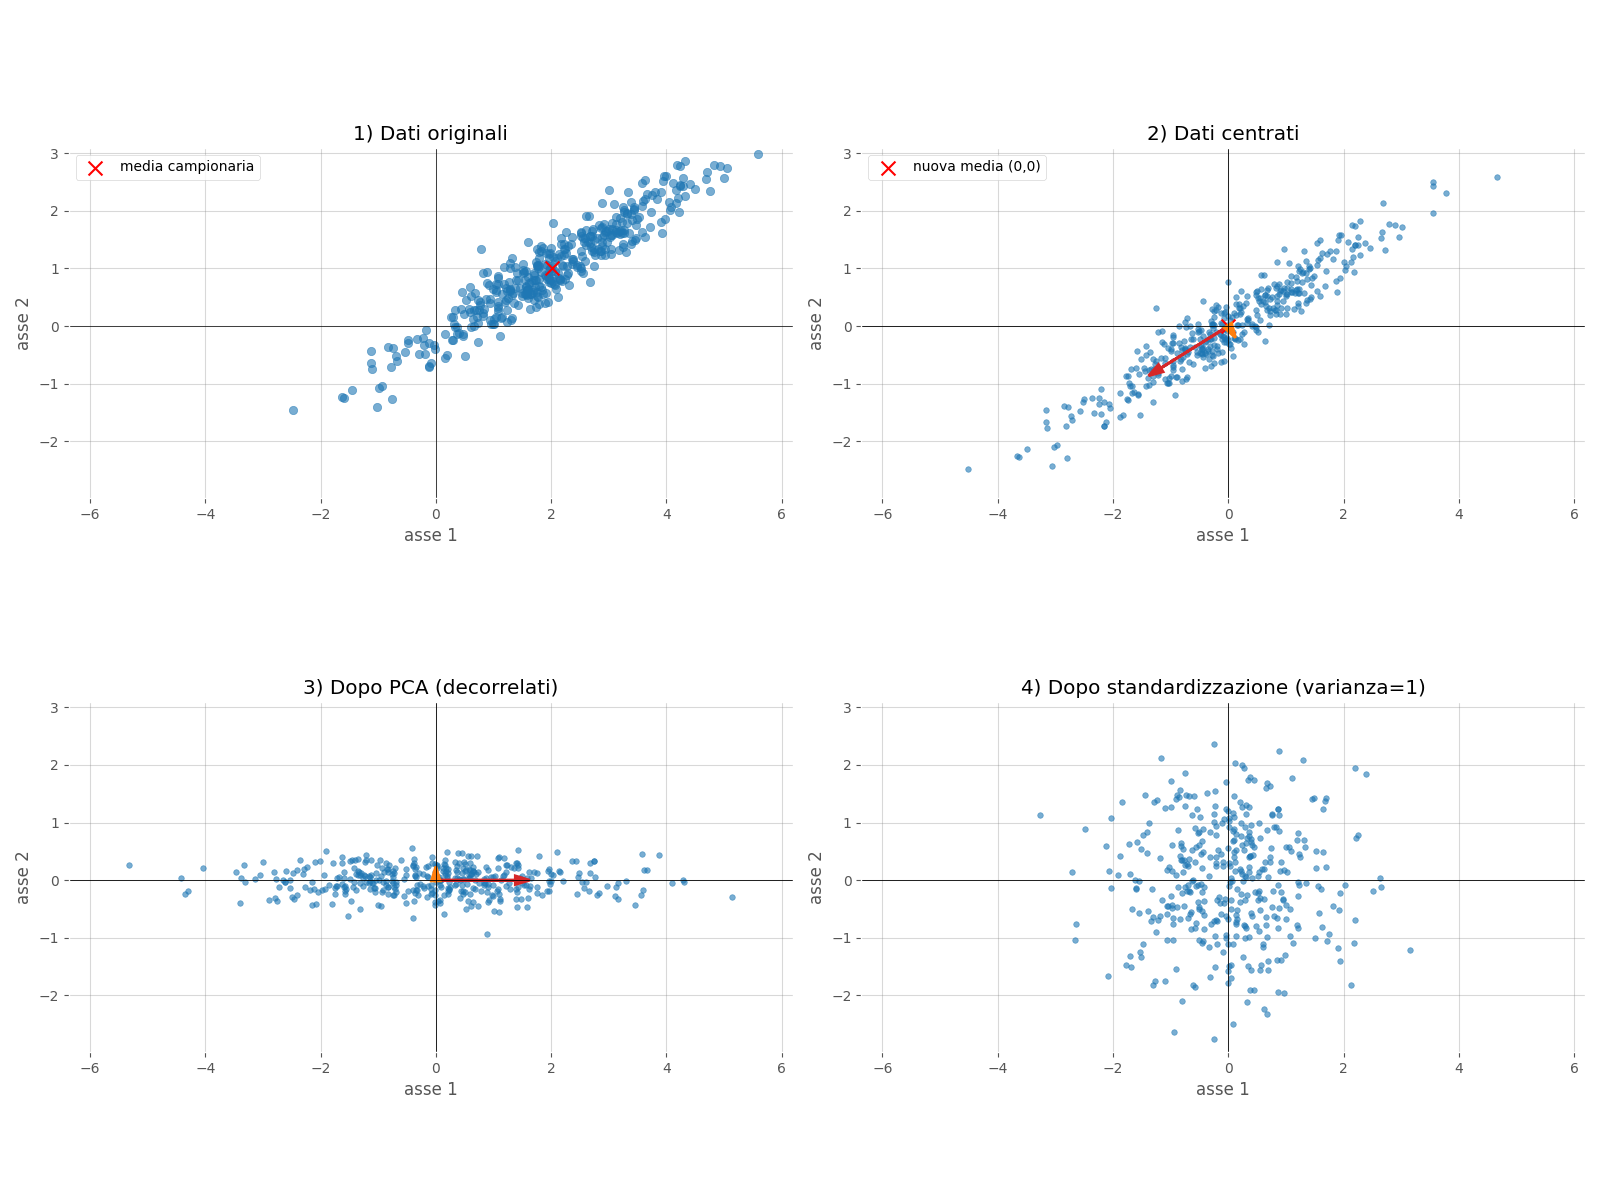
\includegraphics[width=\textwidth]{images/th_10_12/pca_progressione1.png}
    \caption{Esempio di primo approccio alla PCA: 1) Dati originali. 2) Dati centrati. 3) PCA. 4) Dati standardizzati dopo la PCA.}
    \label{fig:pca_progressione1}
\end{figure}

\begin{figure}[H]
    \centering
    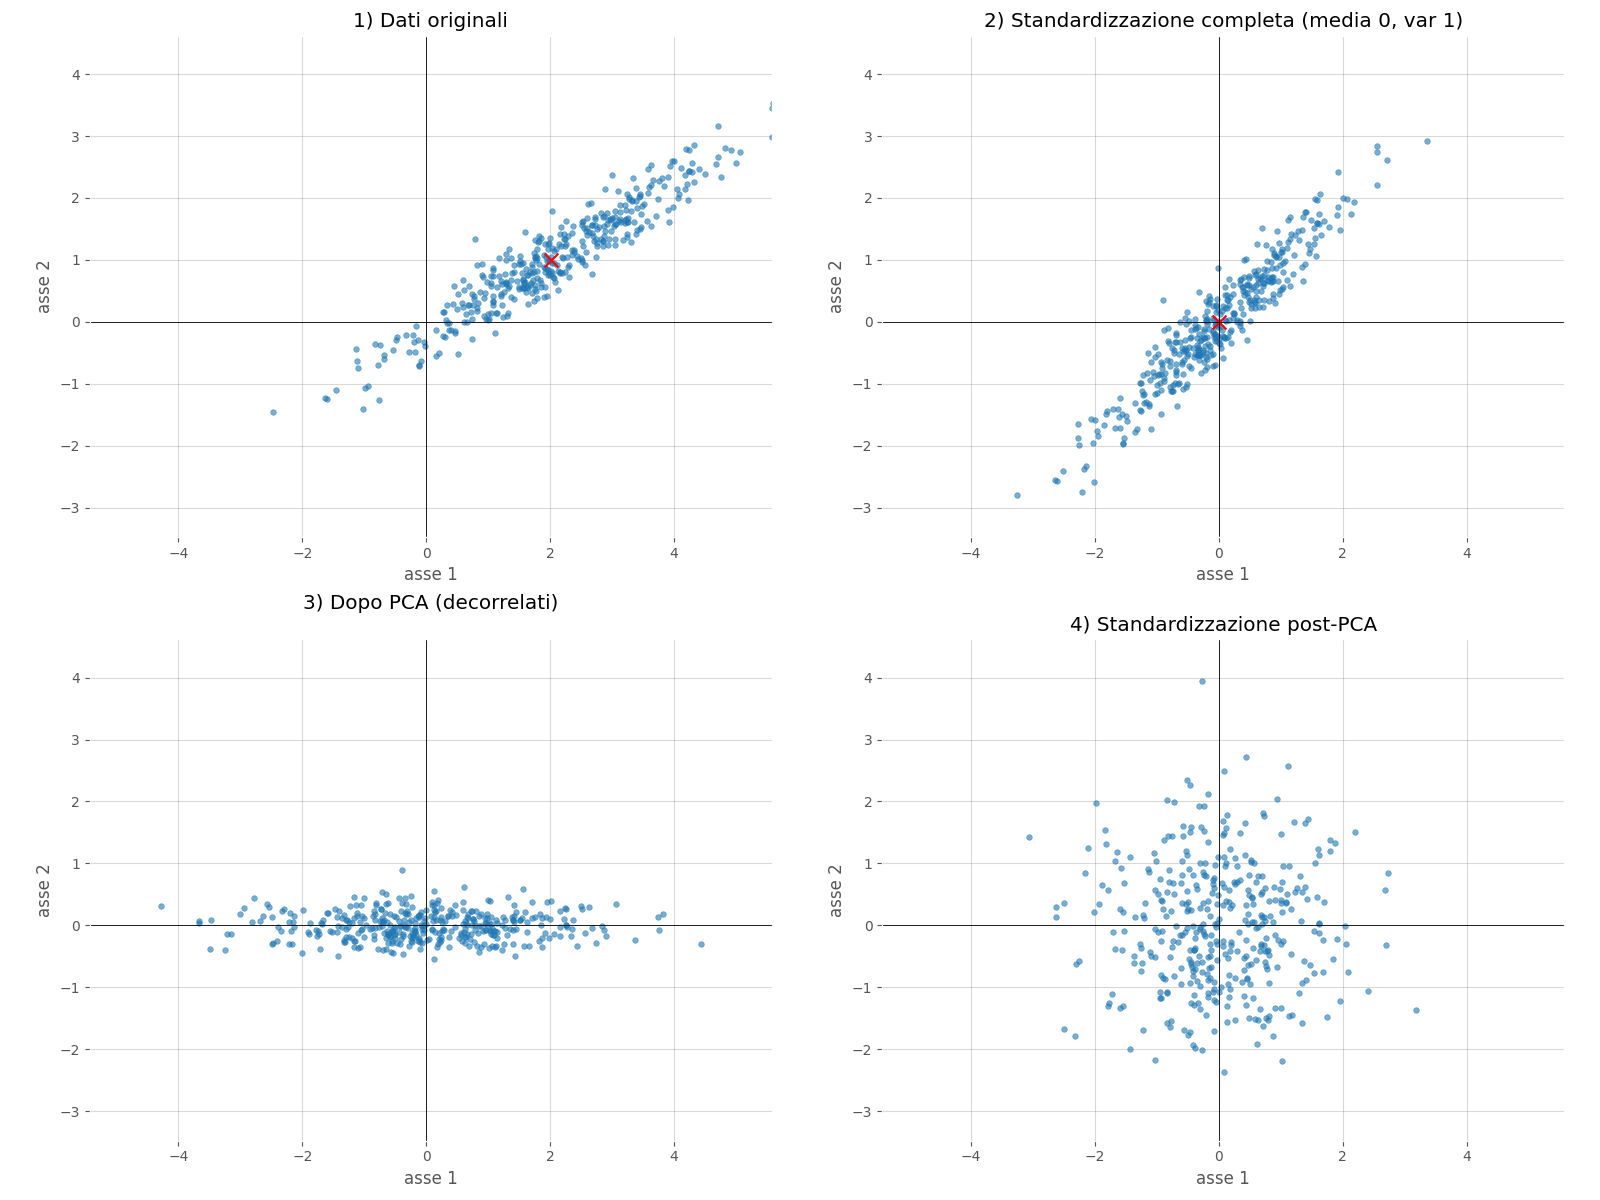
\includegraphics[width=\textwidth]{images/th_10_12/pca_progressione2.png}
    \caption{Esempio di secondo approccio alla PCA: 1) Dati originali. 2) Standardizzazione completa. 3) PCA. 4) Dati standardizzati dopo la PCA.}
    \label{fig:pca_progressione2}
\end{figure}

Questi due approcci corrispondono a:

\begin{itemize}
  \item PCA su \( \Sigma \): privilegia le direzioni di massima varianza
  assoluta;
  \item PCA su matrice di correlazione: privilegia le direzioni di massima
  varianza relativa, indipendente dall'unità di misura.
\end{itemize}

\begin{nota}{Approccio standardizzato}{pca-standard}
Applicare la PCA dopo aver standardizzato equivale a diagonalizzare la matrice
di correlazione \( \rho(X) \), ovvero \( \mathrm{Cov}(Z) \) dove \( Z \) è la
versione standardizzata di \( X \).
\end{nota}

\paragraph{Unità di misura e varianza.}
La matrice di covarianza \( \Sigma = \mathrm{Cov}(X) \) è influenzata
dall’unità di misura delle variabili: se una variabile ha un’unità molto
più grande, avrà anche una varianza più grande, e quindi tenderà a dominare
le componenti principali.

\begin{nota}{Influenza delle unità di misura}{pca-unita}
Se le variabili hanno unità di misura molto diverse (es. altezza in cm, peso in
kg), conviene standardizzare prima della PCA. Altrimenti la componente
principale potrebbe riflettere solo la scala di una variabile.
\end{nota}

\paragraph{Rappresentazione grafica dei due approcci.}

Nella seconda riga viene applicata la standardizzazione prima della PCA: il
risultato finale (dopo PCA) è visivamente diverso. In entrambi i casi si
ottiene una matrice di covarianza diagonale, ma le componenti principali sono
diverse.

\begin{nota}{Quando usare la standardizzazione}{pca-standard-when}
Se non si ha una chiara ragione per dare peso a una variabile più che ad
un'altra (es. tutte hanno importanza comparabile), allora è consigliabile usare
l'approccio con standardizzazione.
\end{nota}



\section{Analisi Fattoriale (Factor Analysis)}\label{sec:factor-analysis}

L'Analisi Fattoriale è una tecnica statistica utilizzata per ridurre il numero
di variabili osservate in un numero inferiore di variabili latenti chiamate
\textbf{fattori}. Mentre la PCA riduce la dimensionalità conservando la
varianza, la Factor Analysis cerca di spiegare le correlazioni tra le variabili
attraverso fattori latenti, e può essere vista come un'estensione della PCA.

\begin{definizione}{Fattori e variabili osservate}{factor-analysis}
Nel modello di Analisi Fattoriale, le variabili osservate \( X_1, X_2, \dots,
X_m \) sono espresse come una combinazione lineare di fattori latenti \( F_1,
F_2, \dots, F_k \) più un errore \( \epsilon_1, \epsilon_2, \dots, \epsilon_m
\):
\[
X_i = \lambda_{i1} F_1 + \lambda_{i2} F_2 + \dots + \lambda_{ik} F_k +
\epsilon_i
\]
dove \( \lambda_{ij} \) è il \textbf{factor loading} che esprime la relazione
tra la variabile osservata \( X_i \) e il fattore \( F_j \).
\end{definizione}

\subsection{Factor Loadings}

I \textbf{factor loadings} \( \lambda_{ij} \) rappresentano il peso di ciascun
fattore latente \( F_j \) sulla variabile osservata \( X_i \). Questi valori
mostrano quanto ciascun fattore contribuisce alla varianza della variabile
osservata. Un alto factor loading indica che la variabile è fortemente
correlata con il fattore.

\begin{esempio}{Factor loadings}{factor-loadings}
Nel caso di due fattori latenti \( F_1 \) e \( F_2 \), i fattori di carico
potrebbero essere:
\[
F_1 = 1.1 X_1 + 0.8 X_2, \quad F_2 = 1.1 X_1 + 0.8 X_2
\]
Ciò significa che \( X_1 \) e \( X_2 \) sono fortemente influenzati da entrambi
i fattori, con pesi \( \lambda_{11} = 1.1 \), \( \lambda_{12} = 0.8 \), e così
via.
\end{esempio}

\subsection{Obiettivo dell'analisi fattoriale}

L'obiettivo dell'Analisi Fattoriale è quello di ridurre il numero di variabili
osservate \( X_1, X_2, \dots, X_m \) in \( k \) fattori \( F_1, F_2, \dots, F_k
\), dove \( k < m \), cercando di mantenere la maggior parte della varianza.
L'analisi si concentra nel trovare i fattori latenti che meglio spiegano le
correlazioni tra le variabili.

\begin{nota}{Riduzione dimensionale nella Factor Analysis}{factor-reduction}
La riduzione di dimensione in Factor Analysis non è come nella PCA, dove si
cerca di massimizzare la varianza, ma si cerca di spiegare le correlazioni tra
le variabili attraverso un numero ridotto di fattori.
\end{nota}

\subsection{Quando usare l'Analisi Fattoriale?}

L'Analisi Fattoriale è utile quando:
\begin{itemize}
  \item Le variabili originali sono fortemente correlate tra loro;
  \item Si vuole ridurre la dimensionalità dei dati senza perdere troppe
  informazioni;
  \item Le variabili sono influenzate da un numero ridotto di fattori latenti.
\end{itemize}

\begin{nota}{Fattori "schiacciati"}{factor-schiacciati}
Quando il numero di variabili osservate \( m \) è grande e ci sono molte
componenti di \( Y \) con varianza piccola, l'Analisi Fattoriale è spesso più
adatta rispetto alla PCA, che potrebbe perdere troppe informazioni in presenza
di molte variabili "schiacciate" (ovvero con bassa varianza).
\end{nota}

\subsection{Relazione con la PCA}

L'Analisi Fattoriale può essere vista come una generalizzazione della PCA.
Mentre la PCA si concentra nel massimizzare la varianza, la Factor Analysis
cerca di spiegare la varianza condivisa tra le variabili attraverso fattori
latenti. Quindi, la PCA può essere considerata come un caso particolare di
Factor Analysis, dove tutti i fattori sono assunti ortogonali e indipendenti.

\subsection{Riduzione dimensionale e scelta del numero di componenti}

Quando \( m \) (il numero di variabili) è grande, esistono molte componenti
principali con varianza piccola. La PCA cerca di ridurre la dimensione del
vettore \( X \) mantenendo la varianza totale e riducendo la complessità del
modello. La somma delle varianze prima e dopo la trasformazione è costante e
conserva la varianza totale:
\[
\text{Var}(X_1) + \dots + \text{Var}(X_m) = \text{Var}(Y_1) + \dots +
\text{Var}(Y_m) = \text{varianza totale}
\]
Questa relazione implica che la traccia della matrice di covarianza \( \Sigma \)
è uguale alla somma degli autovalori di \( \Sigma \), ovvero:
\[
\text{tr}(\Sigma) = \text{tr}(\Lambda)
\]
dove \( \Lambda \) è la matrice diagonale degli autovalori.

\subsubsection{Distribuzione degli autovalori}

Tipicamente, gli autovalori \( \lambda_1 \geq \lambda_2 \geq \dots \geq
\lambda_m > 0 \) sono ordinati in modo decrescente. Questo ordine riflette la
quantità di varianza spiegata da ciascuna componente principale. I componenti
principali con autovalori maggiori spiegano una porzione maggiore della varianza
totale.

Un approccio comune è quello di utilizzare un grafico dei cosiddetti
\textbf{cambiamenti di pendenza} (come lo scree plot \ref{fig:screeplot}) per determinare il numero
di componenti principali da mantenere. Un cambiamento significativo nella
pendenza suggerisce il numero ottimale di componenti da considerare:
Nel grafico sopra, le prime 3 componenti sembrano spiegare la maggior parte
della varianza.

\begin{figure}[H]
    \centering
    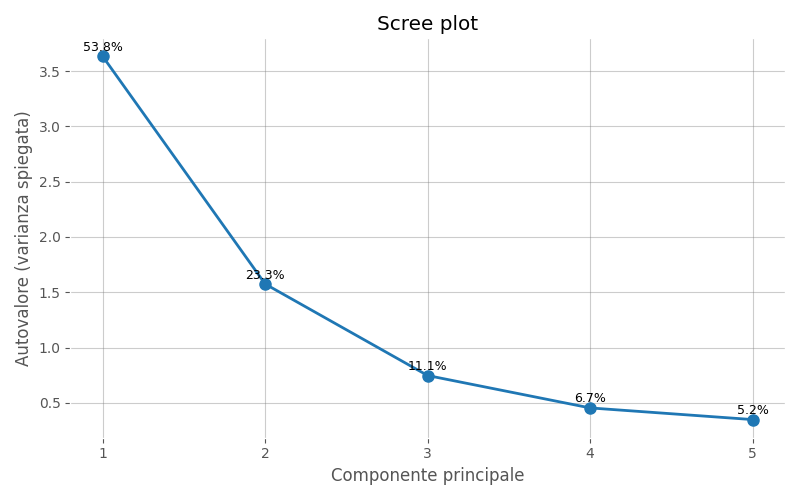
\includegraphics[width=0.6\textwidth]{images/th_10_12/screeplot.png}
    \caption{Esempio di scree plot per la selezione del numero di componenti principali. Si osserva un cambiamento di pendenza significativo dopo la terza componente, suggerendo che le prime tre componenti catturano la maggior parte della varianza.}
    \label{fig:screeplot}
\end{figure}

\subsection{Quando standardizzare i dati}

Quando i dati hanno unità di misura diverse, è importante standardizzarli
prima di applicare la PCA. Questo è cruciale, poiché le variabili con unità
più grandi tenderanno a dominare la varianza, influenzando fortemente le
componenti principali.

Se dopo la PCA i dati non vengono standardizzati, si ottiene una rotazione dei
dati senza alcuna scalatura. In questo caso, la PCA non fornirà una riduzione
della dimensione che tiene conto della varianza relativa di ciascuna variabile,
ma solo una rotazione rispetto alla distribuzione dei dati. Di conseguenza, la
distanza tra i punti sarà influenzata solo dalla loro distribuzione e non dalla
varianza delle variabili.

\begin{nota}{Standardizzazione dopo PCA}{pca-standardizzazione}
Standardizzare i dati prima della PCA è fondamentale per ridurre il rischio di
amplificare il rumore nelle componenti con bassa varianza. La standardizzazione
aiuta a bilanciare l'influenza di variabili con scale diverse.
\end{nota}

\subsection{Effetto della standardizzazione}

Quando i dati vengono standardizzati dopo la PCA, la varianza di ciascuna
componente principale è distribuita in modo più uniforme, evitando che
variabili con bassa varianza distorcano i risultati. Il grafico sottostante
mostra l'effetto della standardizzazione:

Nel grafico:
- \( \mu \) e \( \Sigma \) indicano i dati originali con la loro media e
covarianza,
- \( 0, \Sigma \) indica i dati centrati ma non standardizzati,
- \( 0, I \) rappresenta i dati dopo standardizzazione.

\begin{nota}{Importanza della standardizzazione}{pca-scaling}
La standardizzazione dopo la PCA è essenziale quando le variabili hanno scale
diverse, poiché permette una comparazione equa tra le variabili e riduce
l'influenza di quelle con una varianza maggiore.
\end{nota}

\section{Distribuzioni Multidimensionali Notevoli}

\subsection{Distribuzione Gaussiana Multidimensionale}

La distribuzione Gaussiana (o Normale) Multidimensionale è una delle
distribuzioni di probabilità più importanti in statistica e machine learning.
Essa rappresenta la generalizzazione della distribuzione Gaussiana a vettori
aleatori di più dimensioni.

\begin{definizione}{Gaussiana Multidimensionale}{gaussiana-multi}
Un vettore aleatorio $X = (X_1, X_2, \dots, X_p)$ a valori in $\mathbb{R}^p$
segue una distribuzione Gaussiana Multidimensionale se la sua notazione è
$$
X \sim \mathcal{N}(\mu, \Sigma)
$$
dove:
\begin{itemize}
    \item $\mu \in \mathbb{R}^p$ è il \textbf{vettore media}.
    \item $\Sigma \in M_{p,p}$ è la \textbf{matrice di covarianza}, che deve
    essere simmetrica e semidefinita positiva.
\end{itemize}
\end{definizione}

\begin{nota}{}{gaussiana-params}
I parametri $\mu$ e $\Sigma$ determinano completamente la distribuzione. Il
vettore media $\mu$ definisce il centro della distribuzione, mentre la matrice
di covarianza $\Sigma$ ne definisce la forma e l'orientamento.
\end{nota}

Geometricamente, per $p=2$, la funzione di densità di probabilità (PDF) ha una
forma a campana tridimensionale. Le curve di livello di questa campana sono
ellissi concentriche centrate in $\mu$.

\begin{figure}[H]
    \centering
    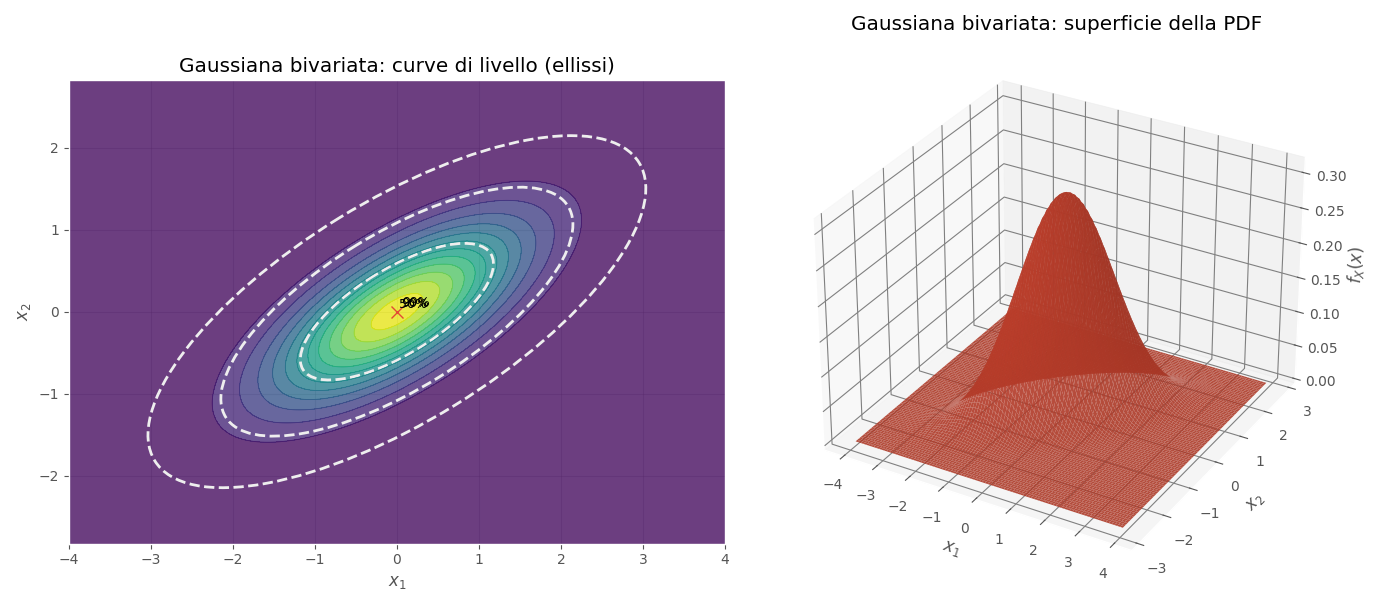
\includegraphics[width=0.6\textwidth]{images/th_10_12/gaussiana_multidimensionale_2d3d.png}
    \caption{Esempio di distribuzione Gaussiana bivariata con media $\mu$ e matrice di covarianza $\Sigma$. Le curve di livello sono ellissi che rappresentano le regioni di uguale densità di probabilità.}
    \label{fig:gaussiana_bivariata}
\end{figure}

\begin{proposizione}{Funzione di Densità di Probabilità (PDF)}{gaussiana-pdf}
Se la matrice di covarianza $\Sigma$ è invertibile (ovvero definita positiva),
allora il vettore aleatorio $X$ ammette una funzione di densità di probabilità
$f_X(x)$ data da:
$$
f_X(x) = \frac{1}{(2\pi)^{p/2} \det(\Sigma)^{1/2}}
\exp\left\{-\frac{1}{2}(x-\mu)^T \Sigma^{-1} (x-\mu)\right\}
$$
Se $\Sigma$ non è invertibile (singolare), la distribuzione è detta
\textbf{degenere} e la massa di probabilità è concentrata su un sottospazio
affine di $\mathbb{R}^p$.
\end{proposizione}

\subsubsection*{Interpretazione della Matrice di Covarianza}

La forma e l'orientamento degli ellissoidi delle curve di livello dipendono
direttamente dalla matrice di covarianza $\Sigma$.

\begin{nota}{}{gaussiana-cov-assi}
Una covarianza nulla tra due componenti, $\text{Cov}(X_i, X_j) = \Sigma_{ij} =
0$, implica che gli assi degli ellissoidi sono paralleli agli assi cartesiani.
\end{nota}

\begin{esempio}{Forma degli Ellissoidi}{gaussiana-ellissoidi}
Analizziamo tre casi per una Gaussiana bivariata ($p=2$) con media $\mu =
\begin{pmatrix} 0 \\ 0 \end{pmatrix}$:
\begin{enumerate}
    \item[\textbf{a.}] \textbf{Covarianza nulla:} Se $\Sigma = \begin{pmatrix}
    \sigma_1^2 & 0 \\ 0 & \sigma_2^2 \end{pmatrix}$, ad esempio $\Sigma =
    \begin{pmatrix} 2 & 0 \\ 0 & 1 \end{pmatrix}$, le componenti $X_1$ e $X_2$
    sono incorrelate. Gli assi degli ellissoidi sono allineati con gli assi
    cartesiani e la loro larghezza è proporzionale a $\sigma_1$ e $\sigma_2$.
    
    \item[\textbf{b.}] \textbf{Covarianza non nulla:} Se $\Sigma =
    \begin{pmatrix} 2 & 1 \\ 1 & 1 \end{pmatrix}$, la covarianza non nulla
    $\Sigma_{12}=1$ indica una correlazione tra $X_1$ e $X_2$. Questo causa una
    rotazione degli ellissoidi: i loro assi principali non sono più paralleli
    agli assi cartesiani.
    
    \item[\textbf{c.}] \textbf{Matrice singolare (degenere):}] Se $\Sigma =
    \begin{pmatrix} 2 & \sqrt{2} \\ \sqrt{2} & 1 \end{pmatrix}$, la matrice non
    è invertibile ($\det(\Sigma) = 2 \cdot 1 - (\sqrt{2})^2 = 0$). Tutta la
    massa di probabilità giace sulla retta $x_1 = \sqrt{2} x_2$. La
    distribuzione non ha una PDF in $\mathbb{R}^2$.
\end{enumerate}
\end{esempio}

Una proprietà fondamentale e unica della distribuzione Gaussiana riguarda la
relazione tra indipendenza e incorrelazione.

\begin{teorema}{Indipendenza e Incorrelazione}{gaussiana-indip-incor}
Per un vettore aleatorio con distribuzione Gaussiana, la condizione di
\textbf{indipendenza} tra le sue componenti è \textbf{equivalente} alla
condizione di \textbf{covarianza nulla} (incorrelazione).
$$
\text{Componenti indipendenti} \iff \text{Covarianza nulla}
$$
\end{teorema}

\begin{nota}{}{gaussiana-indip-impl}
In generale, per altre distribuzioni, vale solo l'implicazione: indipendenza
$\Rightarrow$ covarianza nulla. L'implicazione inversa non è garantita, ma lo
è per la Gaussiana.
\end{nota}

\subsubsection*{Casi Particolari}

\begin{proposizione}{Gaussiana Standard Multidimensionale}{gaussiana-standard}
Se $\mu = \mathbf{0}$ e $\Sigma = I$ (matrice identità), allora le componenti
$X_1, \dots, X_p$ sono Gaussiane standard indipendenti e identicamente
distribuite, $X_i \sim \mathcal{N}(0,1)$ i.i.d.
In questo caso, la PDF ha \textbf{simmetria sferica} (o radiale):
$$
f_X(x) = (2\pi)^{-p/2} \exp\left\{-\frac{1}{2}x^T x\right\} = C \cdot
\exp\left\{-\frac{1}{2}\|x\|^2\right\}
$$
dove $\|x\|^2 = x_1^2 + \dots + x_p^2$ è il quadrato della norma euclidea.
\end{proposizione}

Una conseguenza interessante di questo caso è che la somma dei quadrati di
variabili normali standard indipendenti segue una distribuzione Chi-quadrato.

\begin{nota}{Distribuzione Chi-quadrato}{chi-quadro}
Nel caso di una Gaussiana Standard Multidimensionale, la norma quadra del
vettore $X$, $\|X\|^2$, segue una distribuzione Chi-quadrato con $p$ gradi di
libertà:
$$
\|X\|^2 \sim \chi^2(p)
$$
\end{nota}

Infine, presentiamo una definizione più astratta ma generale, che copre anche i
casi degeneri.

\begin{definizione}{Definizione Astratta}{gaussiana-astratta}
Un vettore aleatorio $X$ ha una legge Gaussiana multivariata in $\mathbb{R}^p$
se e solo se, per ogni vettore $a \in \mathbb{R}^p$, la combinazione lineare $Y
= a^T X$ ha una legge Gaussiana univariata su $\mathbb{R}$ o è una costante
deterministica.
\end{definizione}

\subsection{Distribuzione Multinomiale}

La distribuzione multinomiale è la generalizzazione della distribuzione
binomiale. Mentre un esperimento binomiale consiste in $n$ prove indipendenti
con due possibili esiti (successo/insuccesso), un esperimento multinomiale
consiste in $n$ prove indipendenti, ciascuna con $m$ possibili esiti.

\begin{definizione}{Multinomiale}{multinomiale}
Un vettore aleatorio $X = (X_1, X_2, \dots, X_m)$ segue una distribuzione
Multinomiale con parametri $n$ (numero di prove) e $p$ (vettore di
probabilità), e si scrive:
$$
X \sim \text{Multin}(n, p)
$$
dove:
\begin{itemize}
    \item $X_i$ conta il numero di volte che si è verificato l'esito $i$ nelle
    $n$ prove.
    \item $p = (p_1, p_2, \dots, p_m)$ è un vettore di probabilità, con $p_i$
    che rappresenta la probabilità dell'esito $i$.
\end{itemize}
Devono valere i seguenti vincoli: $\sum_{i=1}^{m} p_i = 1$ e $\sum_{i=1}^{m} X_i
= n$.
\end{definizione}

\begin{nota}{}{multinomiale-dipendenza}
Le componenti del vettore $X = (X_1, \dots, X_m)$ sono \textbf{dipendenti},
poiché la loro somma è fissata a $n$. Tuttavia, la distribuzione marginale di
ogni singola componente $X_i$ è una binomiale: $X_i \sim \text{Bin}(n, p_i)$.
\end{nota}

\begin{proposizione}{Funzione di Massa di Probabilità (PMF)}{multinomiale-pmf}
La funzione di massa di probabilità (PMF) della distribuzione multinomiale è
data da:
$$
P(X_1=x_1, \dots, X_m=x_m) = \frac{n!}{x_1! x_2! \dots x_m!} p_1^{x_1} p_2^{x_2}
\dots p_m^{x_m}
$$
dove $\sum_{i=1}^{m} x_i = n$. Il termine frazionario è noto come
\textbf{coefficiente multinomiale} e conta il numero di modi in cui $n$ oggetti
possono essere partizionati in $m$ gruppi di numerosità $x_1, \dots, x_m$.
\end{proposizione}

\begin{esempio}{Coefficiente Multinomiale}{multinomiale-coeff}
Quanti sono gli anagrammi della parola "STATISTICA"?
La parola è lunga $n=10$ caratteri. Le frequenze delle lettere sono: S (2), T
(3), A (2), I (2), C (1).
Il numero di anagrammi è dato dal coefficiente multinomiale:
$$
\binom{10}{2, 3, 2, 2, 1} = \frac{10!}{2! \cdot 3! \cdot 2! \cdot 2! \cdot 1!} =
75600
$$
\end{esempio}


\subsection{Distribuzione di Dirichlet}

La distribuzione di Dirichlet è una distribuzione di probabilità continua per
un vettore di numeri reali positivi che sommano a 1. È spesso descritta come
una "distribuzione su distribuzioni", ed è il coniugato a priori della
distribuzione Multinomiale nell'inferenza Bayesiana.

\begin{definizione}{Dirichlet}{dirichlet}
Un vettore aleatorio $X = (X_1, \dots, X_m)$ a valori in $\mathbb{R}^m$ segue
una distribuzione di Dirichlet con parametro di concentrazione $\alpha =
(\alpha_1, \dots, \alpha_m)$, con $\alpha_i > 0$. Si scrive:
$$
X \sim \text{Dirichlet}(\alpha)
$$
Il vettore $X$ è tale per cui $X_i \in [0, 1]$ per ogni $i$, e $\sum_{i=1}^{m}
X_i = 1$.
\end{definizione}

Geometricamente, il dominio (o supporto) della distribuzione di Dirichlet è un
\textit{simplesso standard}. Per $m=3$, è un triangolo equilatero nello spazio
3D, come mostrato nelle figure di esempio.

\begin{proposizione}{Funzione di Densità di Probabilità (PDF)}{dirichlet-pdf}
La funzione di densità di probabilità della distribuzione di Dirichlet è:
$$
f_X(x) = C_\alpha \prod_{i=1}^{m} x_i^{\alpha_i - 1}
$$
definita sul simplesso $x_i \ge 0$ e $\sum x_i = 1$. $C_\alpha$ è una costante
di normalizzazione che dipende dalla funzione Gamma.
\end{proposizione}


\begin{figure}[H]
    \centering
    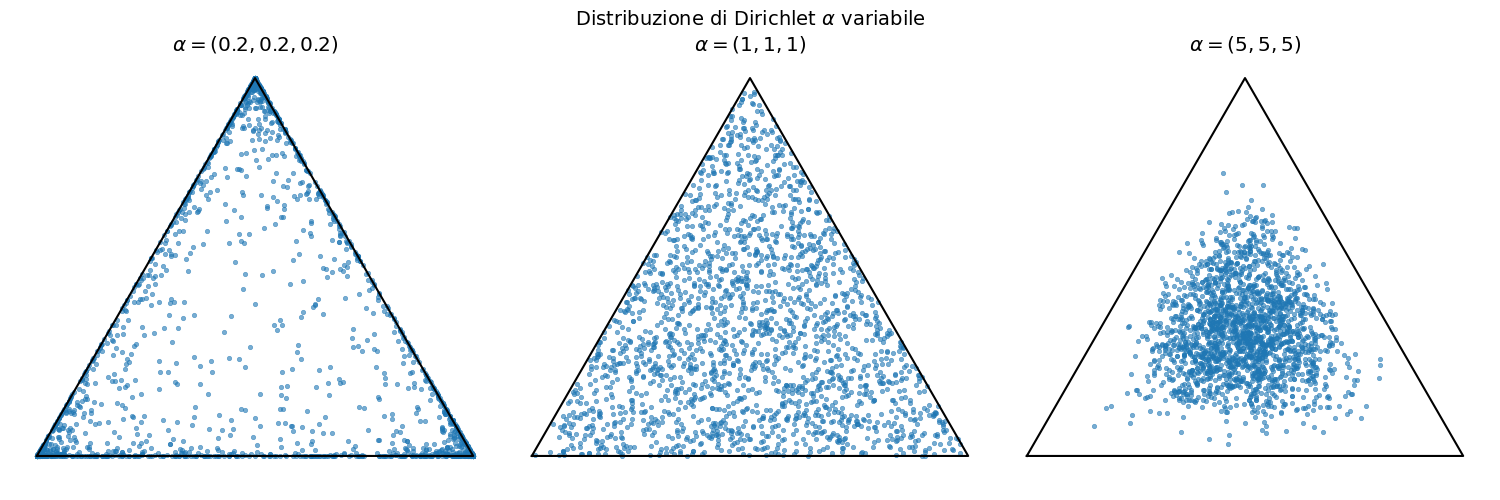
\includegraphics[width=\textwidth]{images/th_10_12/dirichlet.png}
    \caption{Esempio di distribuzione di Dirichlet tramite simplesso 2D. Le regioni colorate rappresentano diverse modalità della distribuzione.}
    \label{fig:dirichlet}
\end{figure}

\begin{proposizione}{Valore Atteso}{dirichlet-valore-atteso}
Il valore atteso di un vettore $X \sim \text{Dirichlet}(\alpha)$ è:
$$
E[X_i] = \frac{\alpha_i}{\sum_{j=1}^{m} \alpha_j} \implies E[X] = \frac{1}{S}
\alpha
$$
dove $S = \sum_{j=1}^{m} \alpha_j$.
\end{proposizione}

\begin{nota}{Relazione con la distribuzione Beta}{dirichlet-beta}
Per $m=2$, la distribuzione di Dirichlet è equivalente alla distribuzione Beta.
$$
\text{Dirichlet}(\alpha_1, \alpha_2) \equiv \text{Beta}(\alpha_1, \alpha_2)
$$
Inoltre, se $X_1 \sim \text{Unif}(0,1)$ (che è una $\text{Beta}(1,1)$) e $X_2 =
1 - X_1$, allora il vettore $(X_1, X_2) \sim \text{Dirichlet}(1, 1)$.
\end{nota}

I parametri $\alpha_i$ controllano la forma della distribuzione. Valori di
$\alpha_i < 1$ spingono la massa di probabilità verso i vertici del simplesso.
Valori di $\alpha_i > 1$ spingono la massa verso il centro. Se tutti gli
$\alpha_i$ sono uguali, la distribuzione è simmetrica. Se sono diversi, la
distribuzione è sbilanciata verso il vertice corrispondente all' $\alpha_i$
più grande.
